\documentclass{article}
\usepackage{graphicx} % Required for inserting images
\usepackage[english,russian]{babel}

\title{Лабораторная работа 2}
\author{Крыжановский Максим Сергеевич}
\date{April 2024}

\begin{document}

\maketitle

\section{Introduction}

В рамках задания было необходимо разработать метод определения и классификации треугольных деревянных объектов из игрового набора, а также реализовать это в виде программы.

\section{Программная реализация}
Программа была написана на языке Python с использованием фреймворка PyQt5. В программу можно загружать изображение, производить различные преобразования, а также по нажатию кнопки определить все деревянные структуры на картинке, их координаты и классификацию.

\section{Данные}
Для работы над этим заданием предлагалось исследовать различные фотографии с изображенными на них фигурами. В углах каждой фигуры находились точки для определения класса этой точки.

\begin{figure}[h!]
    \centering
    \includegraphics[width=0.9\linewidth]{3_images.png}
    \caption{Примеры входных данных}
    \label{fig:enter-label}
\end{figure}

При исследовании данных было решено попробовать сегментацию Кэнни, а также различные цветные фильтры, так как точки на игровых фигурах были разных цветов. Также можем посмотреть на распределение цветов на картинке, разложив ее на три канала.

\begin{figure}[h!]
    \centering
    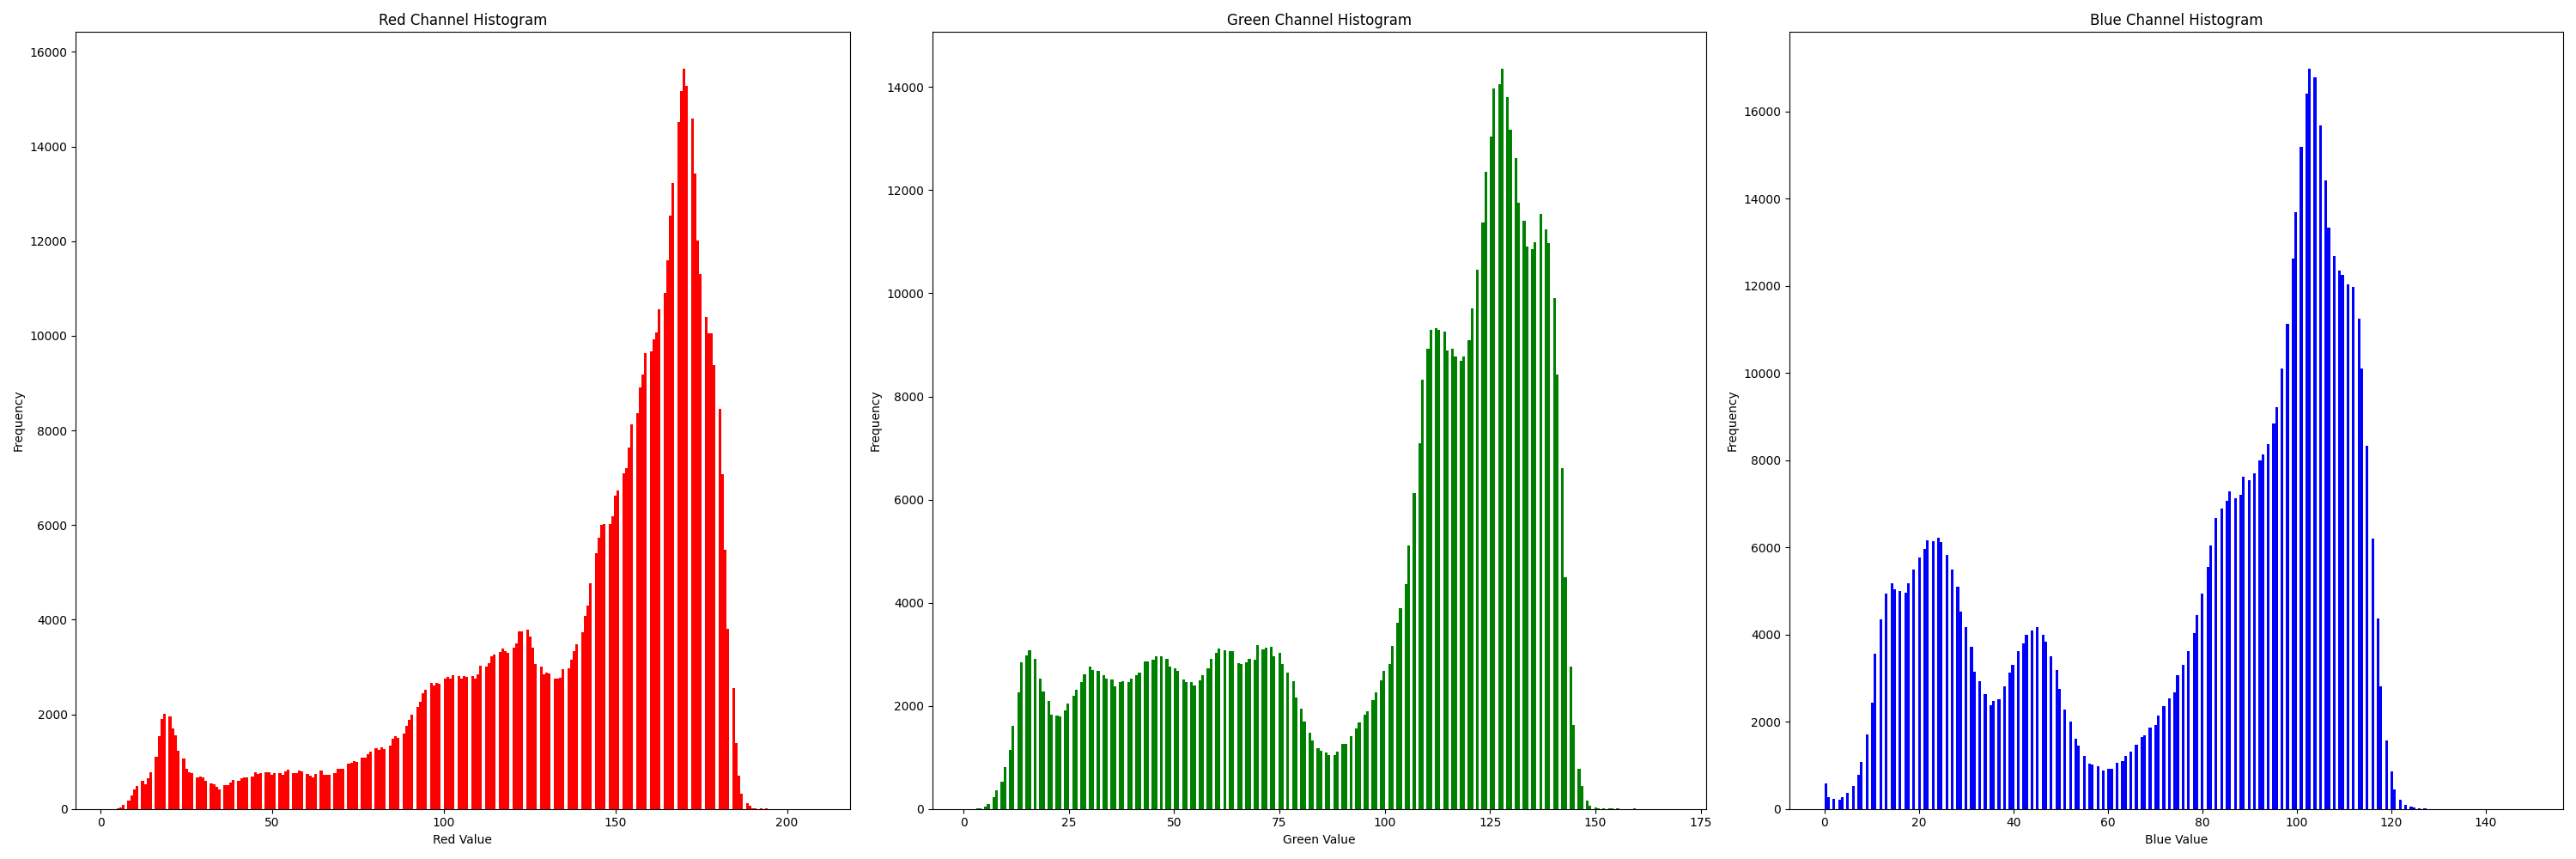
\includegraphics[width=0.75\linewidth]{rgb_histogram.png}
    \caption{Частоты каждого цветового канала}
    \label{fig:enter-label}
\end{figure}

\section{Алгоритм выделения треугольников}
Для обнаружения границ был использован алгоритм Кэнни, работающий следующим образом:
\begin{enumerate}
    \item Предварительная обработка: Изображение сначала преобразуется в оттенки серого, если оно не было таковым. Это обеспечивает одноканальное изображение, что упрощает дальнейшую обработку.
    \item Удаление шума: Применяются различные методы сглаживания (например, фильтр Гаусса), чтобы уменьшить шум на изображении. Это позволяет получить более чистое изображение и улучшить точность обнаружения границ.
    \item Вычисление градиента интенсивности: Затем вычисляются градиенты интенсивности на изображении. Это делается с помощью оператора Собеля или других методов. Градиенты показывают направление и силу изменения интенсивности пикселей на изображении.
    \item Подавление не-максимумов: В этом шаге применяется алгоритм, который подавляет все пиксели, которые не являются локальными максимумами в направлении градиента. Это помогает сохранить только настоящие границы, игнорируя шум и другие непринадлежащие границам детали.
    \item Пороговая обработка: Затем применяется пороговая обработка для определения, какие пиксели являются границами высокой интенсивности (сильные границы), а какие - низкой интенсивности (слабые границы). Это помогает разделить границы на более четкие и менее четкие.
    \item Связывание границ: Наконец, используется метод связывания границ (например, методы трассировки областей), чтобы объединить слабые границы с сильными и получить полные границы объектов на изображении.
\end{enumerate}

\begin{figure}[h!]
    \centering
    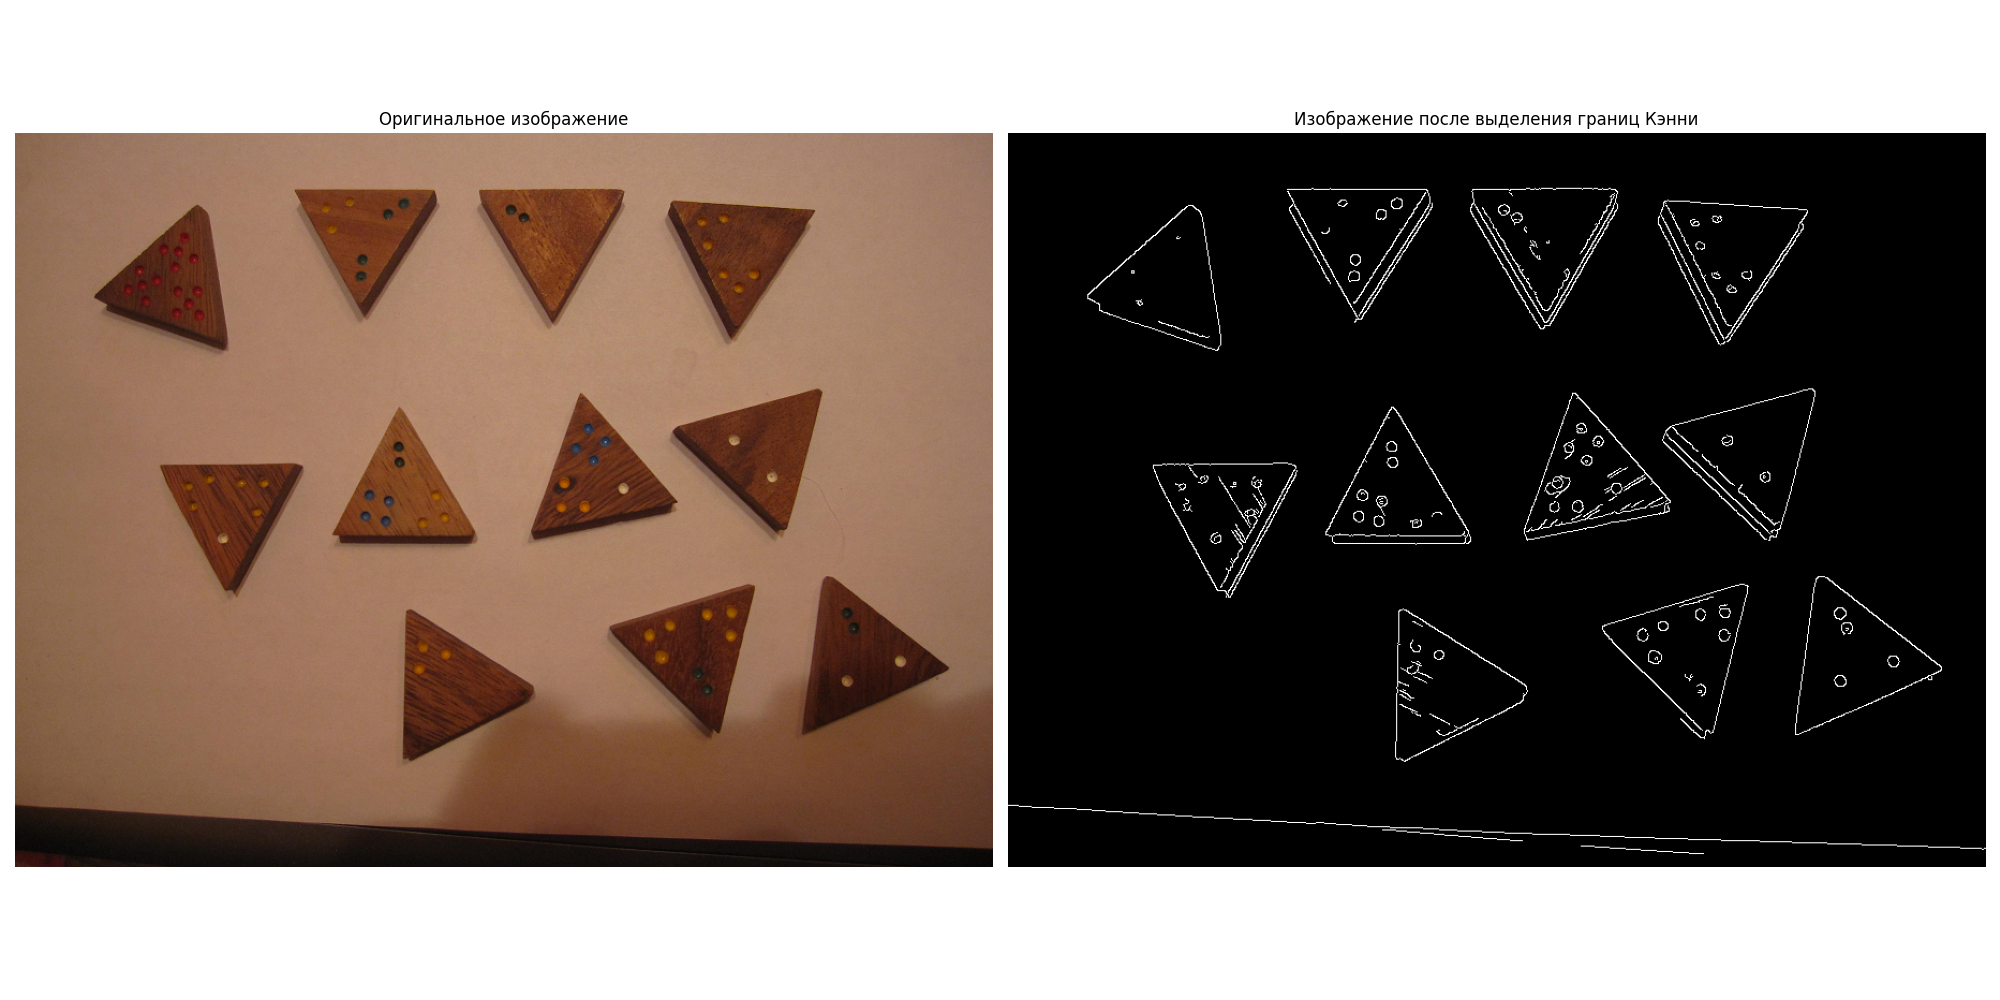
\includegraphics[width=0.9\linewidth]{canny_exp.png}
    \caption{Результат применения поиска границ Canny}
    \label{fig:enter-label}
\end{figure}

После того как были определены границы с помощью алгротма Кэнни производится отбор нужных фигур. В рамках решения задачи необходимо было определить треугольники, поэтому искались именно эти фигуры. Отбор объектов по их форме производился с помощью алгоритма Дугласа-Пекера. 

Для определения центров треугольников считалось среднее между положениями всех пикселей, который входили в компонент связаности. Далее приведем результат того, что у нас получилось.

\begin{figure}
    \centering
    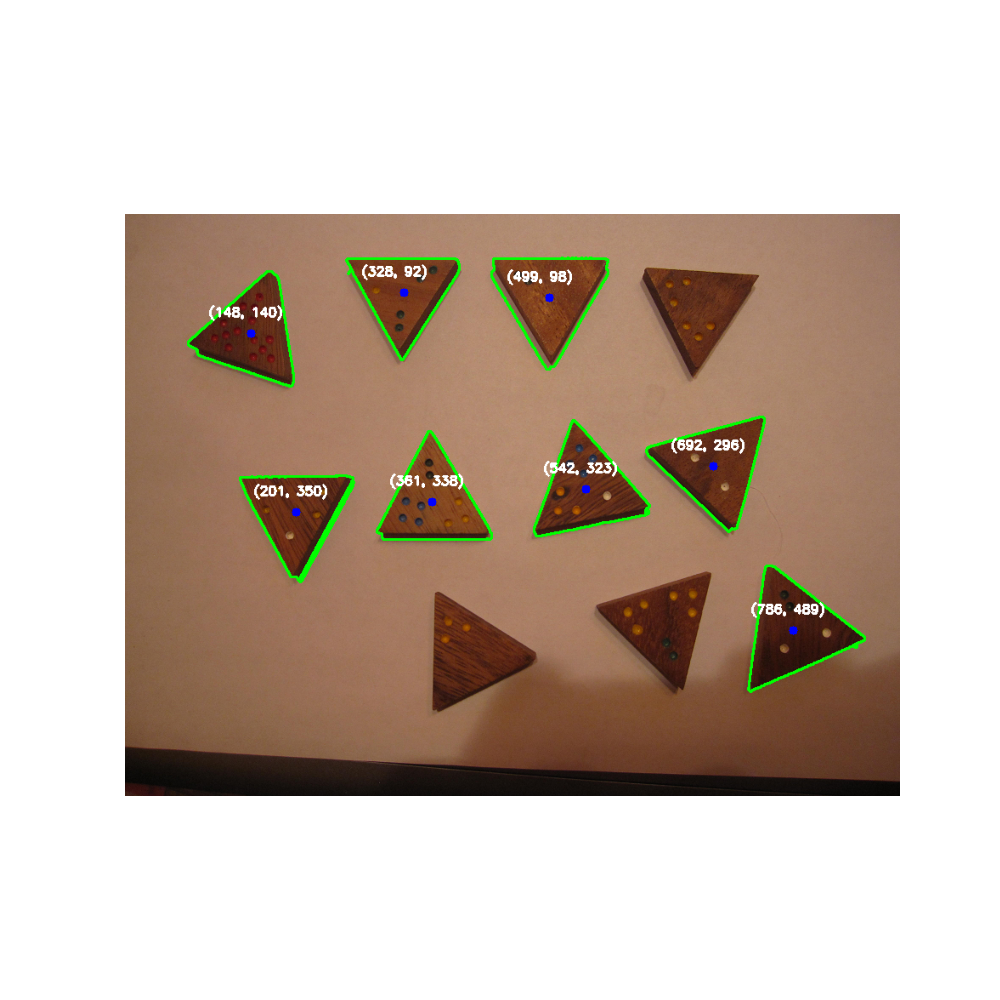
\includegraphics[width=0.9\linewidth]{triangle.png}
    \caption{Результат нахождения центров треугольников}
    \label{fig:enter-label}
\end{figure}

Для определения точек был использован следующий алгоритм:

\begin{enumerate}
    \item Выделение трех каналов изображения - красного, зеленого и голубого
    \item Увеличение контраста на каждом канале
    \item Поиск границ с использованием алгоритма Кэнни на каждом канале
    \item Определение формы границ каждой фигуры и отбор круглых (почти круглых) фигур
\end{enumerate}

Далее необходимо было определить к какой вершине относятся данные точки. На основе проведенного ранее анализа данных было решено обратить внимание на использование цветных фильтров и разложение картинки по цветам для выделения точек, так как они являются самыми контрастными в пределах каждой вершины. Для этого был использован следующий алгоритм. 

\begin{enumerate}
    \item Определение точек внутри каждого найденного контура треугольника
    \item Поиск ближайших к каждой вершине точек определенных внутри контура
    \item Постановка метки
\end{enumerate}

Далее приведем результат работы алгоритма (Рис. 5).

\begin{figure}
    \centering
    \includegraphics[width=0.75\linewidth]{Снимок экрана 2024-04-25 в 00.15.33.png}
    \caption{Установка количества точек в каждой вершине}
    \label{fig:enter-label}
\end{figure}

\section{Выводы}
В целом по работе могу сказать, что алгороитм выделения границ треугольника сработал отсноительно неплохо. Возможно я не успел подобрать наилучшие параметры для сегментации Кэнни, тогда бы согл отображаться более менее все фигуры. Проблема была только с уровнем эксперт, где некоторые фигуры сливались с задним фоном и не проходили фильтр по форме. С определением точек все пошло не очень, потому что так нормально их определить и не получилось. Алгоритм точно требует доработки и, как минимум, правильной настройки или поиска других вариантов определения форм.

\end{document}
